\documentclass[11pt]{article}

% template oficial da disciplina
\usepackage{if69d-template}

% pacotes
\usepackage[brazil]{babel}
\usepackage[utf8]{inputenc}
\usepackage{graphicx}
\usepackage{amsthm,amsfonts,amsmath}
\usepackage{booktabs}
\usepackage[font=footnotesize,
			labelfont=it,
			labelformat=simple]{subcaption}
\renewcommand\thesubfigure{(\alph{subfigure})}

% capa
\instituicao{Universidade Tecnológica Federal do Paraná -- UTFPR -- Campus Curitiba}
\departamento{Departamento Acadêmico de Eletrônica -- DAELN}
\curso{Bacharelado em Sistemas de Informação / Engenharia Eletrônica}
\disciplina{IF69D e OPEET014 -- Processamento Digital de Imagens}
\semestre{2026.2}
\professor{Gustavo B. Borba e Humberto R. Gamba}

\titulo{OMR Exam Grader: Correção Automática de Folhas de Respostas por Reconhecimento Óptico de Marcas}

\autor{Rômulo Barbosa da Silva}{UTFPR}
\autordois{Guilherme Oliver}{UTFPR}
\date{nov.2026}

\begin{document}

\maketitle

\section{Objetivo}

Implementar em Python um sistema completo de Reconhecimento Óptico de Marcas (\textit{Optical Mark Recognition} -- OMR) para correção automática de folhas de respostas de múltipla escolha (50 questões $\times$ 5 alternativas e até 4 tipos de prova) adquiridas por câmera de smartphone, contemplando geração da folha em PDF, pré-processamento, binarização, detecção de marcadores fiduciais, retificação projetiva por homografia, leitura adaptativa das bolhas e atribuição de nota ponderada.

\section{Fundamentação Teórica}

O Reconhecimento Óptico de Marcas (OMR) consiste em detectar a presença ou ausência de marcações feitas a caneta ou lápis em posições pré-determinadas de um formulário impresso~\cite{gonzalez2018}. Quando a aquisição é realizada por câmera de smartphone sem suporte fixo, a imagem capturada sofre três classes principais de degradação: (i) distorção projetiva (perspectiva, rotação e escala); (ii) iluminação não-uniforme e sombras; e (iii) ruído do sensor óptico e granulação do papel.

\subsection{Pré-processamento, Filtragem e Normalização de Iluminação}

Dada uma imagem colorida $I_{\text{RGB}}(x,y)$, converte-se inicialmente para níveis de cinza $I(x,y) \in [0, 255]$. Para atenuar o ruído de alta frequência antes da segmentação, aplica-se um filtro passa-baixas Gaussiano ($G_\sigma * I$) ou, na presença de ruído impulsivo do tipo sal-e-pimenta, o filtro não-linear da mediana em vizinhança $k \times k$~\cite{gonzalez2018}.

Sob iluminação desigual causada pela sombra do smartphone, a intensidade observada pode ser modelada pelo produto entre a iluminância $L(x,y)$ (variação espacial lenta) e a refletância do papel/tinta $R(x,y)$ (variação rápida). Estima-se o fundo claro do papel $\hat{L}(x,y)$ por meio do operador morfológico de fechamento com elemento estruturante elíptico $B$ de raio superior ao das bolhas e letras, conforme a equação~(\ref{eq:bg_norm})~\cite{gonzalez2018}:
\begin{equation} \label{eq:bg_norm}
I_{\text{norm}}(x,y) = \min\!\left(255,\; 255 \cdot \frac{I(x,y)}{(I \bullet B)(x,y)}\right), \quad \text{onde } (I \bullet B) = (I \oplus B) \ominus B.
\end{equation}

Na etapa de binarização, comparam-se duas abordagens clássicas: a limiarização global ótima de Otsu~\cite{otsu1979}, que maximiza a variância interclasses $\sigma_B^2(T)$ do histograma global, e a limiarização local adaptativa Gaussiana~\cite{bradley2007}, na qual o limiar local $T(x,y)$ é dado pela média ponderada Gaussiana $\mu_W(x,y)$ numa janela $W \times W$ subtraída de uma constante $C$:
\begin{equation} \label{eq:adaptive}
B(x,y) = \begin{cases}
255, & \text{se } I_{\text{norm}}(x,y) < \mu_W(x,y) - C \\
0,   & \text{caso contrário.}
\end{cases}
\end{equation}

\subsection{Morfologia, Componentes Conexos e Retificação por Homografia}

Para localizar a folha no espaço, imprimem-se quatro marcadores fiduciais quadrados sólidos nos cantos da área útil. Sobre a imagem binária $B(x,y)$, aplica-se abertura morfológica para eliminar traços finos e executa-se a rotulação de componentes conexos com conectividade-8~\cite{gonzalez2018}. Cada componente candidato $k$ é filtrado por área $A_k$, razão de aspecto $w_k / h_k \approx 1$ e solidez $\mathcal{S}_k = A_k / A_{\text{hull},k} \ge 0{,}72$.

Obtidos os quatro centroides detectados $\mathbf{p}_i = [x_i, y_i, 1]^T$ na foto e suas coordenadas canônicas conhecidas no modelo da folha $\mathbf{p}'_i = [x'_i, y'_i, 1]^T$ ($i \in \{\text{TL, TR, BR, BL}\}$), estima-se a matriz de transformação projetiva (homografia) $\mathbf{H} \in \mathbb{R}^{3\times 3}$ com 8 graus de liberdade pela equação~(\ref{eq:homography})~\cite{hartley2004}:
\begin{equation} \label{eq:homography}
\lambda_i \begin{bmatrix} x'_i \\ y'_i \\ 1 \end{bmatrix} = \begin{bmatrix} h_{11} & h_{12} & h_{13} \\ h_{21} & h_{22} & h_{23} \\ h_{31} & h_{32} & h_{33} \end{bmatrix} \begin{bmatrix} x_i \\ y_i \\ 1 \end{bmatrix}.
\end{equation}
A imagem retificada $I_{\text{ret}}(x',y')$ é reconstruída por mapeamento inverso (\textit{inverse mapping}) com interpolação bilinear na resolução canônica de $1680 \times 2376$~pixels ($8\text{ px/mm}$ em folha A4).

\subsection{Amostragem das Bolhas e Decisão de Marcação Calibrada}

No referencial canônico retificado, cada bolha da questão $q \in \{1,\dots,50\}$ e alternativa $o \in \{A,B,C,D,E\}$ possui centro $(c_x, c_y)$ e raio $r$ conhecidos. Para evitar que o anel impresso da própria bolha contamine a leitura, define-se uma máscara circular interna $\mathcal{M}_{q,o}$ de raio $r_{\text{int}} = 0{,}74\,r$ e calcula-se a razão de preenchimento (\textit{fill ratio}) $\rho_{q,o}$ conforme a equação~(\ref{eq:fill_ratio}):
\begin{equation} \label{eq:fill_ratio}
\rho_{q,o} = \frac{1}{|\mathcal{M}_{q,o}|} \sum_{(x',y') \in \mathcal{M}_{q,o}} \frac{B_{\text{ret}}(x',y')}{255} \in [0, 1].
\end{equation}

Como pelo menos $75\%$ das 250 bolhas de uma folha correspondem a alternativas não marcadas, os $65\%$ menores valores de $\rho_{q,o}$ na própria folha estimam a média $\mu_{\text{vazia}}$ e o desvio padrão $\sigma_{\text{vazia}}$ do fundo, calibrando o limiar $\tau_{\text{folha}}$ entre o modo das bolhas vazias e a mediana das bolhas preenchidas (com piso mínimo $\tau_{\min} = 0{,}22$). Questões sem nenhuma alternativa com $\rho_{q,o} \ge \tau_{\text{folha}}$ são classificadas como \textbf{em branco}; questões com duas ou mais alternativas acima do limiar são invalidadas por \textbf{dupla marcação}.

\section{Implementação}

O sistema foi implementado em Python~3 de forma modular no repositório \texttt{omr-exam-grader}, utilizando as primitivas de baixo nível do OpenCV~\cite{bradski2000} e NumPy para as operações matriciais, além do ReportLab para geração vetorial da Folha de Respostas (FR) em PDF. A Figura~\ref{fig:pipeline} ilustra o resultado prático das etapas sequenciais do pipeline sobre uma imagem de teste com inclinação projetiva, rotação e gradiente de sombra.

\begin{figure}[!htb]
	\centering
	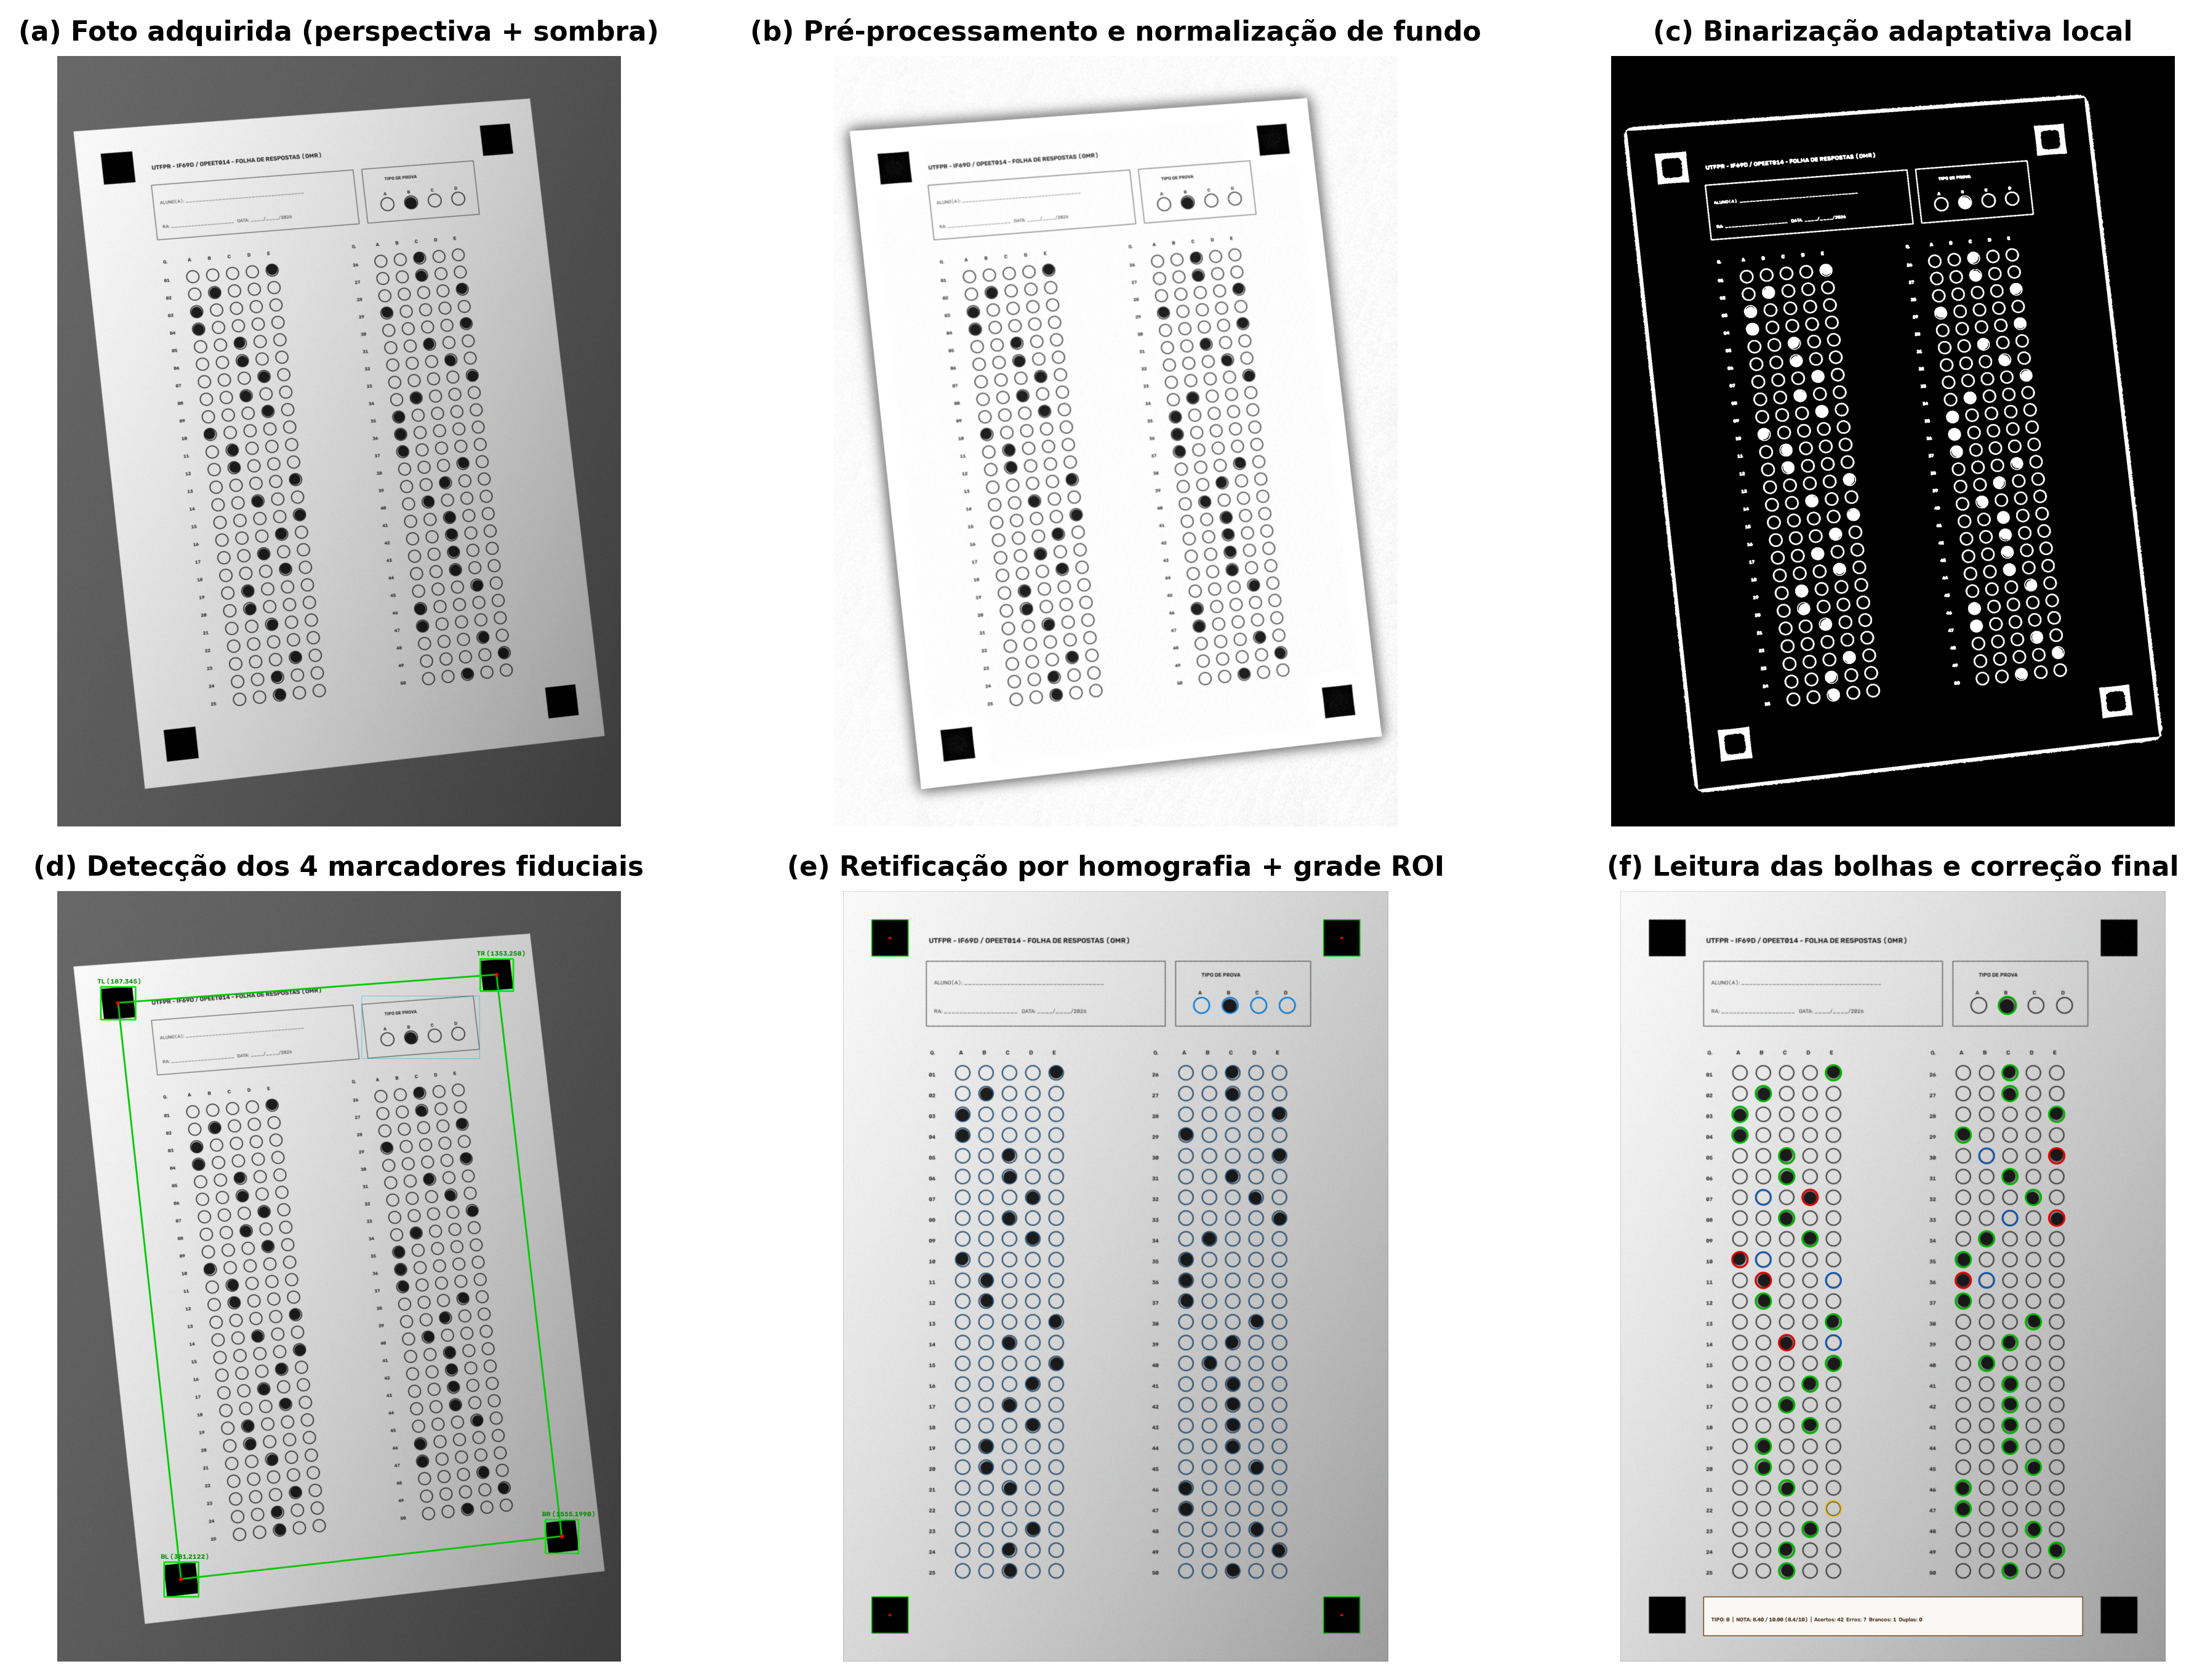
\includegraphics[width=0.96\textwidth]{figuras/fig_pipeline_etapas.png}
	\caption{Etapas do pipeline OMR implementado: (a) foto adquirida com distorção projetiva e sombra; (b) normalização morfológica de iluminação; (c) binarização adaptativa; (d) detecção dos 4 marcadores fiduciais; (e) retificação por homografia e grade canônica de ROIs ($50 \times 5$); (f) leitura das marcas e correção anotada.}
	\label{fig:pipeline}
\end{figure}

Os arquivos entregues organizam-se nos seguintes módulos:
\begin{itemize}
\item \textbf{Núcleo do Pipeline (\texttt{src/omr/})}: \texttt{sheet.py} (geometria canônica A4 a $8\text{ px/mm}$); \texttt{preprocess.py} (filtros Gaussiano/mediana, divisão morfológica de fundo e binarização Otsu/Adaptativa); \texttt{markers.py} (morfologia, componentes conexos e validação do quadrilátero convexo); \texttt{rectify.py} (homografia via \texttt{cv2.findHomography} e \texttt{cv2.warpPerspective}); \texttt{bubbles.py} (amostragem com máscara circular interna e calibração automática de $\tau_{\text{folha}}$); \texttt{grade.py} (gabaritos para tipos A--D, pesos por questão e diagnóstico visual); \texttt{pipeline.py} e \texttt{cli.py} (execução em linha de comando).
\item \textbf{Ferramentas, Interface e Testes (\texttt{tools/}, \texttt{tests/}, \texttt{app.py})}: \texttt{tools/generate\_sheet.py} (gera o PDF \texttt{data/templates/answer\_sheet.pdf} e gabaritos JSON); \texttt{tools/synthetic\_dataset.py} (simulador fotométrico e projetivo com \textit{ground truth}); \texttt{tools/evaluate.py} (experimentos quantitativos); \texttt{app.py} (interface interativa em Streamlit para demonstração ao vivo); e \texttt{tests/test\_omr\_pipeline.py} (testes automatizados com \texttt{pytest}).
\end{itemize}

\section{Resultados e conclusões}

A avaliação quantitativa foi conduzida sobre um conjunto de benchmark de 30 folhas completas ($1.500$ questões e $7.500$ bolhas avaliadas) submetidas a variações combinadas de rotação ($\pm 15^\circ$), escala ($0{,}72$ a $0{,}94$), distorção projetiva de perspectiva, gradiente direcional de sombra (até $50\%$), variação na pressão da caneta e ruído aditivo. A Tabela~\ref{tab:metricas} sintetiza o desempenho global obtido pelo pipeline.

\begin{table}[!htb]
	\centering
	\caption{Desempenho quantitativo global do sistema OMR sobre o conjunto de avaliação ($N = 30$ folhas, $1.500$ questões, $7.500$ bolhas).}
	\label{tab:metricas}
	\vspace{4pt}
	\begin{tabular}{lc}
		\toprule
		\textbf{Métrica Avaliada} & \textbf{Resultado Obtido} \\
		\midrule
		Taxa de detecção dos 4 marcadores fiduciais & $100{,}00\%$ (30 / 30) \\
		Erro médio de localização dos cantos (RMSE) & $1{,}36\text{ pixels}$ ($\approx 0{,}17\text{ mm}$) \\
		Acurácia de identificação do Tipo de Prova (A--D) & $100{,}00\%$ (30 / 30) \\
		Acurácia de leitura por bolha individual ($N = 7.500$) & $100{,}00\%$ ($\text{F1-Score} = 100{,}00\%$) \\
		Acurácia de decisão por questão ($N = 1.500$, incl.\ brancos e duplas) & $100{,}00\%$ \\
		\bottomrule
	\end{tabular}
\end{table}

A Figura~\ref{fig:otsu_adap} apresenta o comparativo entre a limiarização global de Otsu aplicada diretamente sobre a imagem suavizada e a combinação de normalização morfológica de fundo com limiarização adaptativa local. Observa-se na Figura~\ref{fig:otsu_adap}(b) que, sob sombreamento superior a $30\%$, o limiar único de Otsu classifica toda a região sombreada da página como tinta (primeiro plano), degradando severamente a acurácia (Figura~\ref{fig:otsu_adap}(d)). Em contrapartida, a normalização de fundo aliada ao limiar adaptativo mantém $100\%$ de acurácia mesmo quando a sombra reduz a iluminância local em mais de $70\%$.

\begin{figure}[!htb]
	\centering
	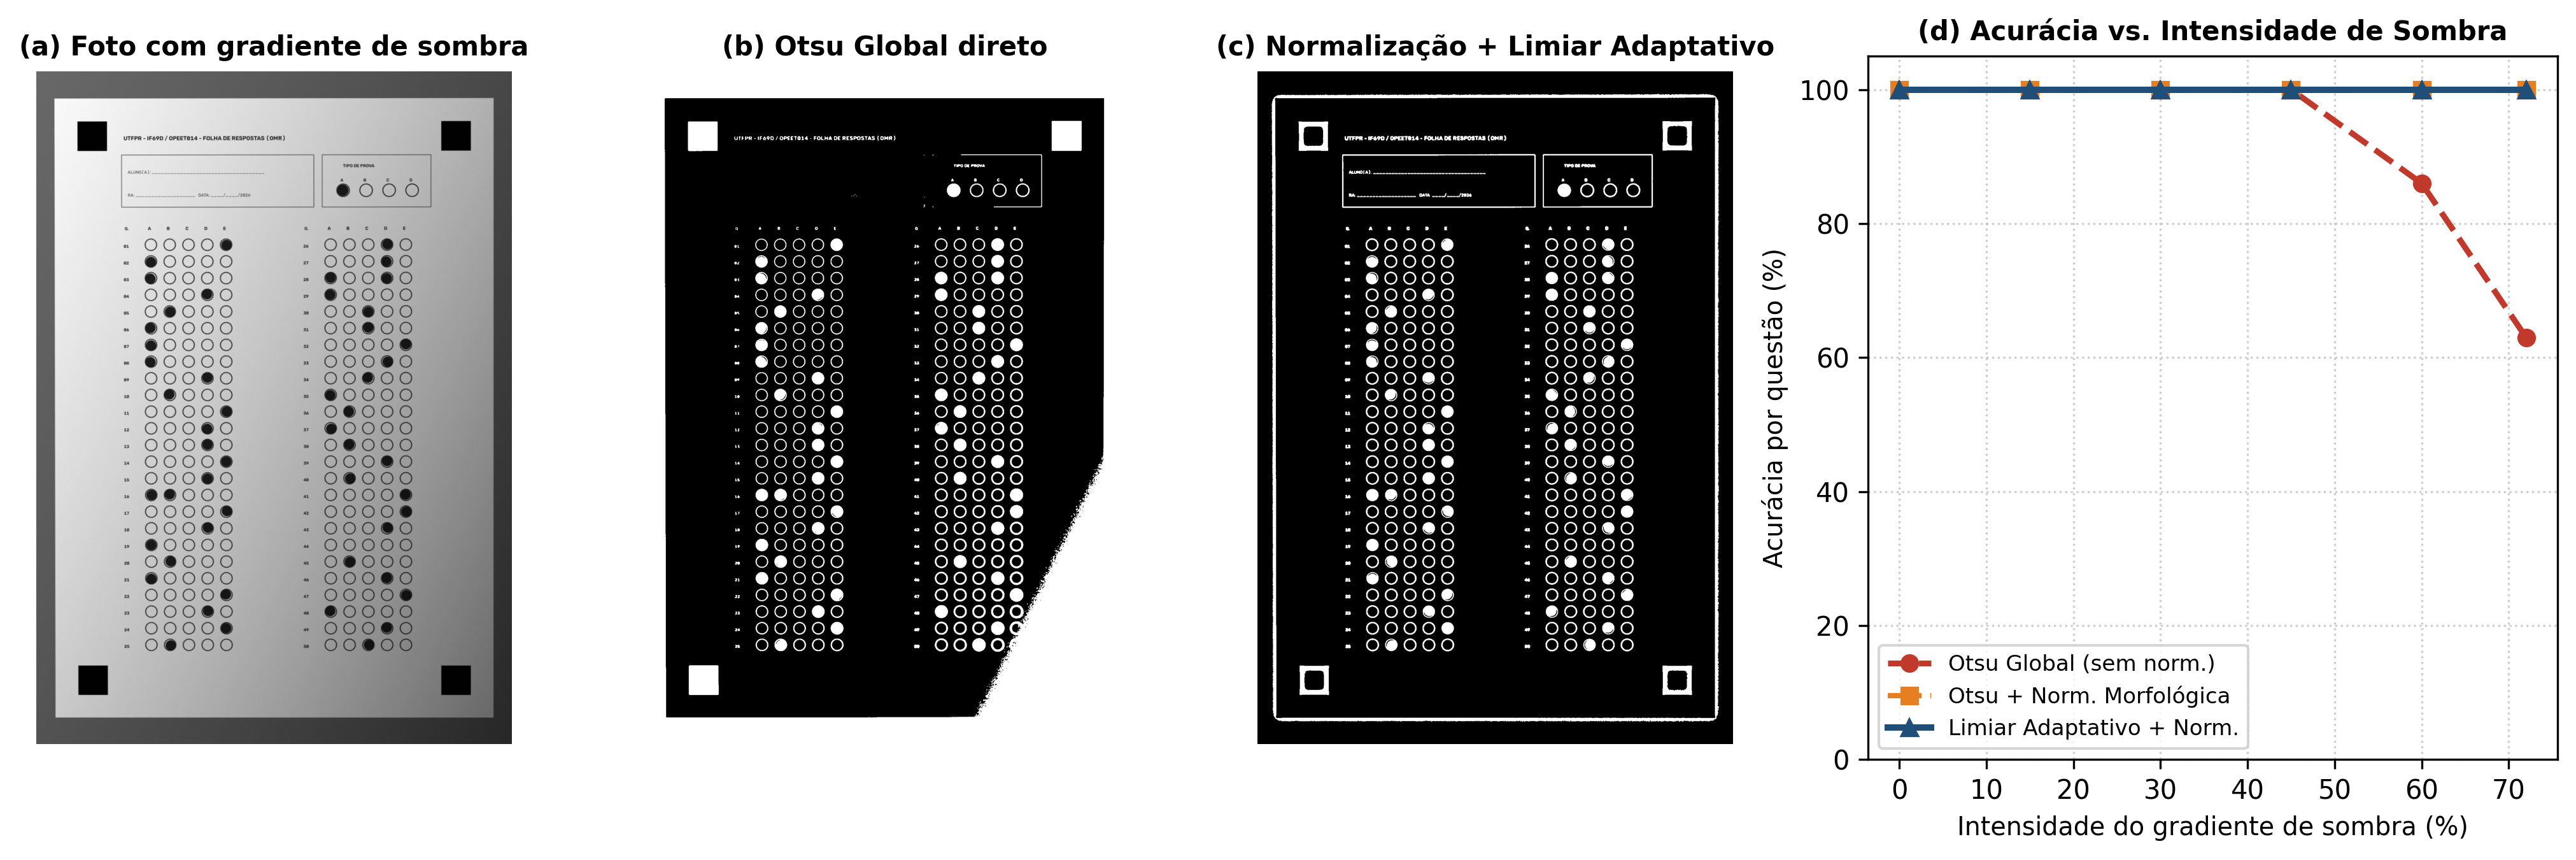
\includegraphics[width=0.98\textwidth]{figuras/fig_otsu_vs_adaptativo.png}
	\caption{Comparação entre Otsu Global e Limiarização Adaptativa sob iluminação não-uniforme: (a) folha com forte gradiente de sombra ($62\%$); (b) falha do Otsu global direto; (c) segmentação correta com normalização morfológica + limiar adaptativo; (d) curva de acurácia em função da intensidade da sombra.}
	\label{fig:otsu_adap}
\end{figure}

As matrizes de confusão por bolha e por questão (incluindo as classes \textit{Branco} e \textit{Dupla marcação}) são apresentadas na Figura~\ref{fig:confusao}, confirmando a ausência de falsos positivos ou falsos negativos nas $7.500$ bolhas testadas. Na Figura~\ref{fig:robustez}, avaliam-se os limites operacionais do algoritmo sob degradações extremas: o sistema mantém $100\%$ de acurácia para rotações de até $25^\circ$, escalas entre $55\%$ e $95\%$ e ruído Gaussiano com $\sigma \le 35$. No experimento de ruído impulsivo sal-e-pimenta (Figura~\ref{fig:robustez}(d)), comprova-se a superioridade teórica do filtro não-linear da mediana ($5\times 5$), que preserva $100\%$ de acurácia até $8\%$ de pixels corrompidos, enquanto o filtro linear Gaussiano sofre degradação progressiva por espalhar os impulsos para dentro das máscaras de amostragem.

\begin{figure}[!htb]
	\centering
	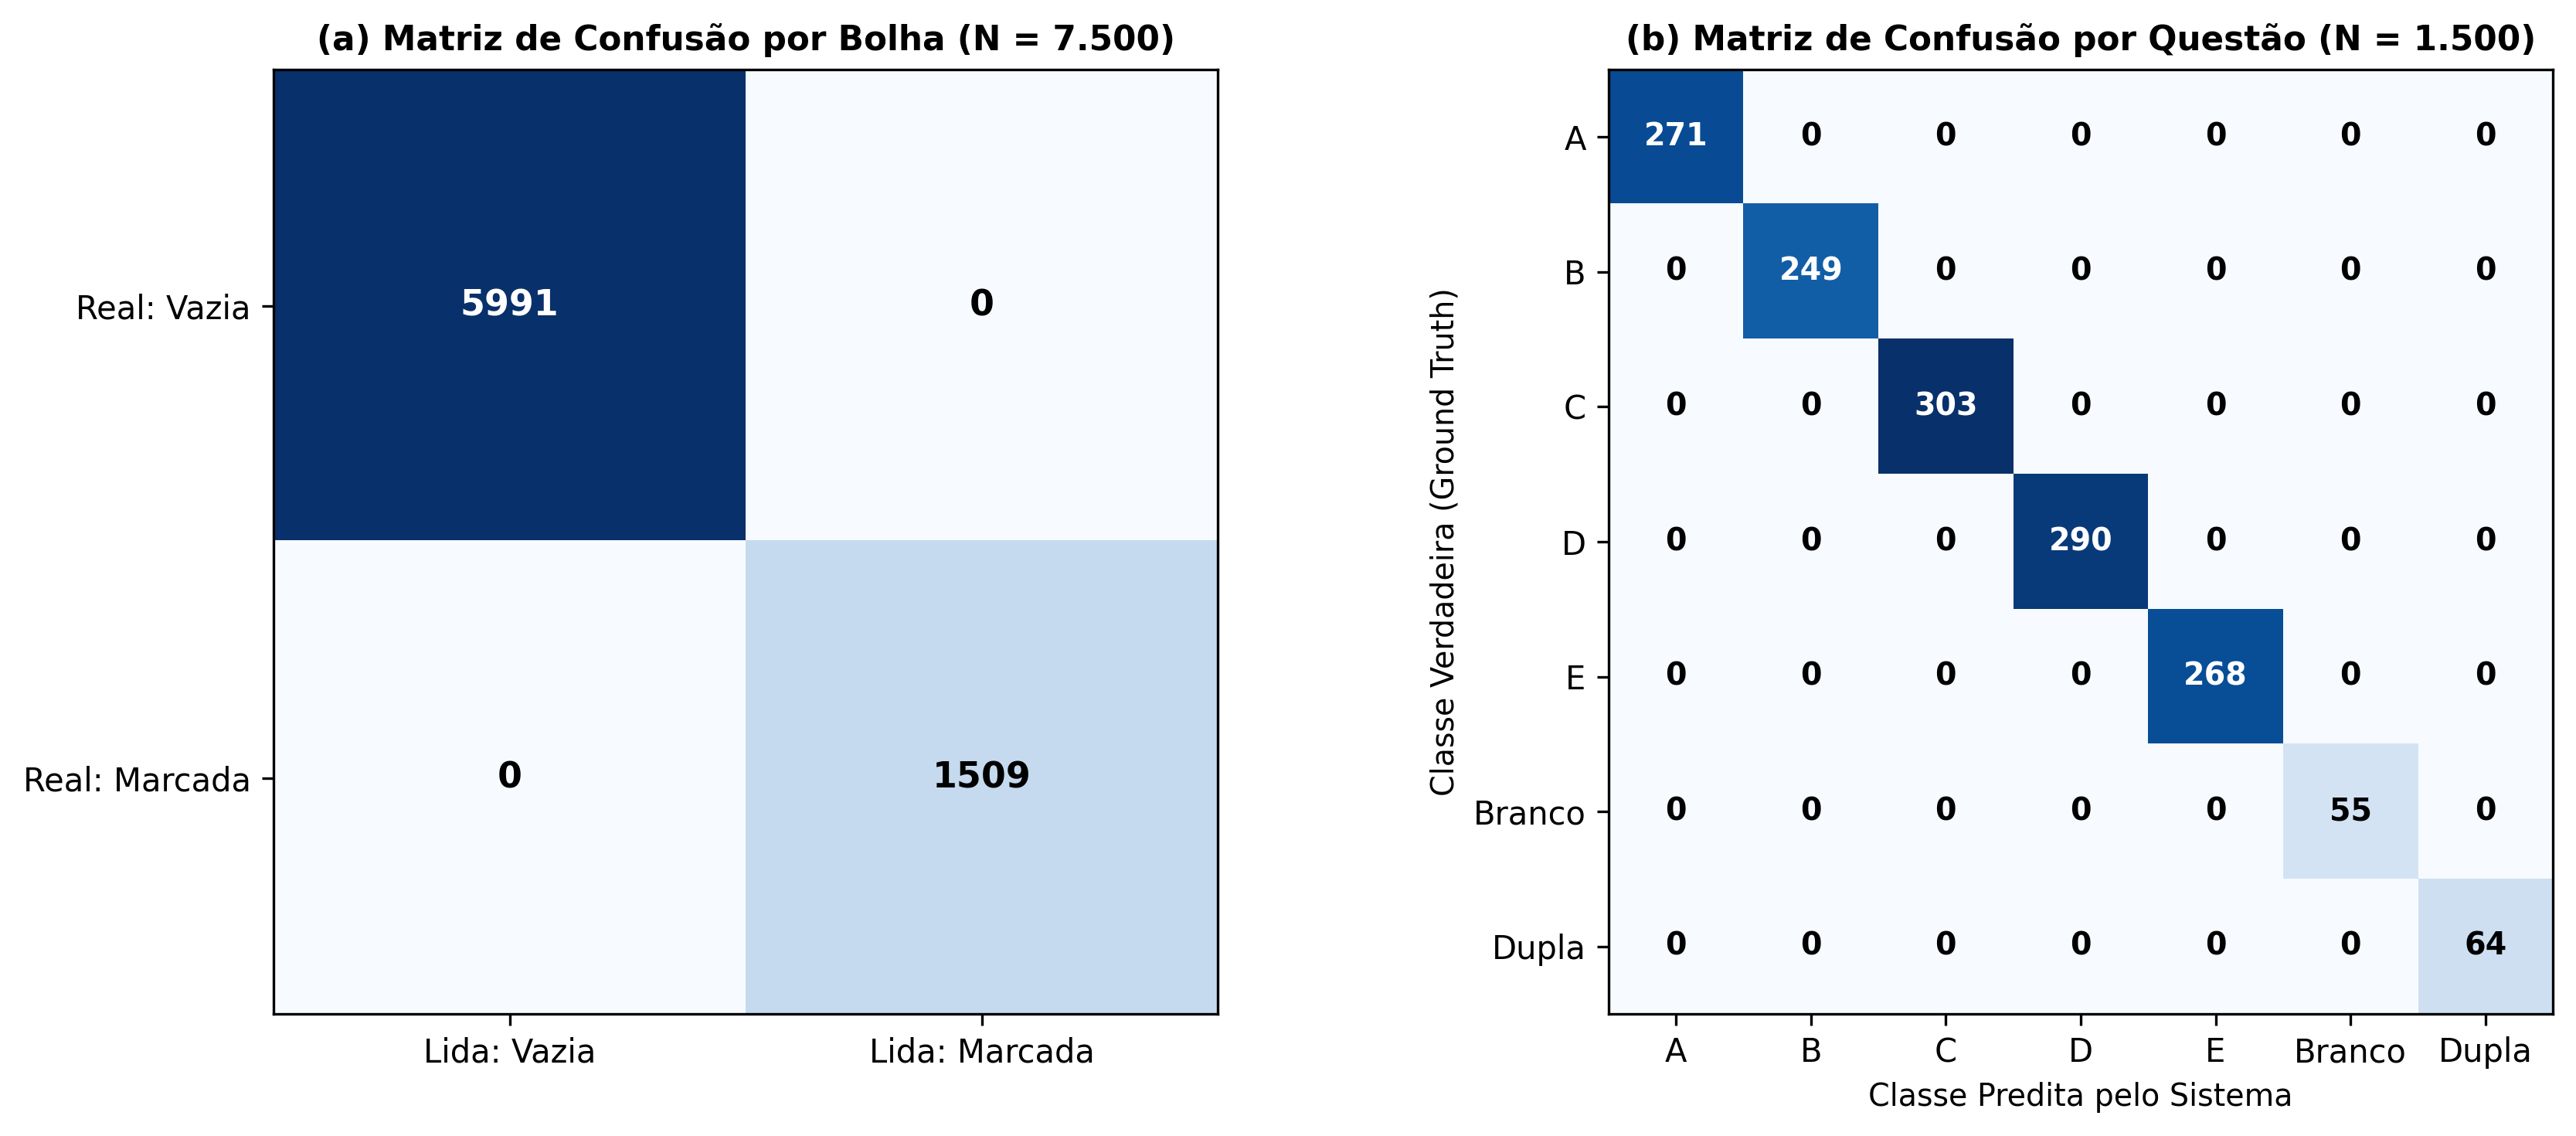
\includegraphics[width=0.92\textwidth]{figuras/fig_matriz_confusao.png}
	\caption{Matrizes de confusão sobre o lote de 30 folhas degradadas: (a) nível de bolha ($N = 7.500$); (b) nível de questão ($N = 1.500$, discriminando alternativas A--E, questões em branco e duplas marcações).}
	\label{fig:confusao}
\end{figure}

\begin{figure}[!htb]
	\centering
	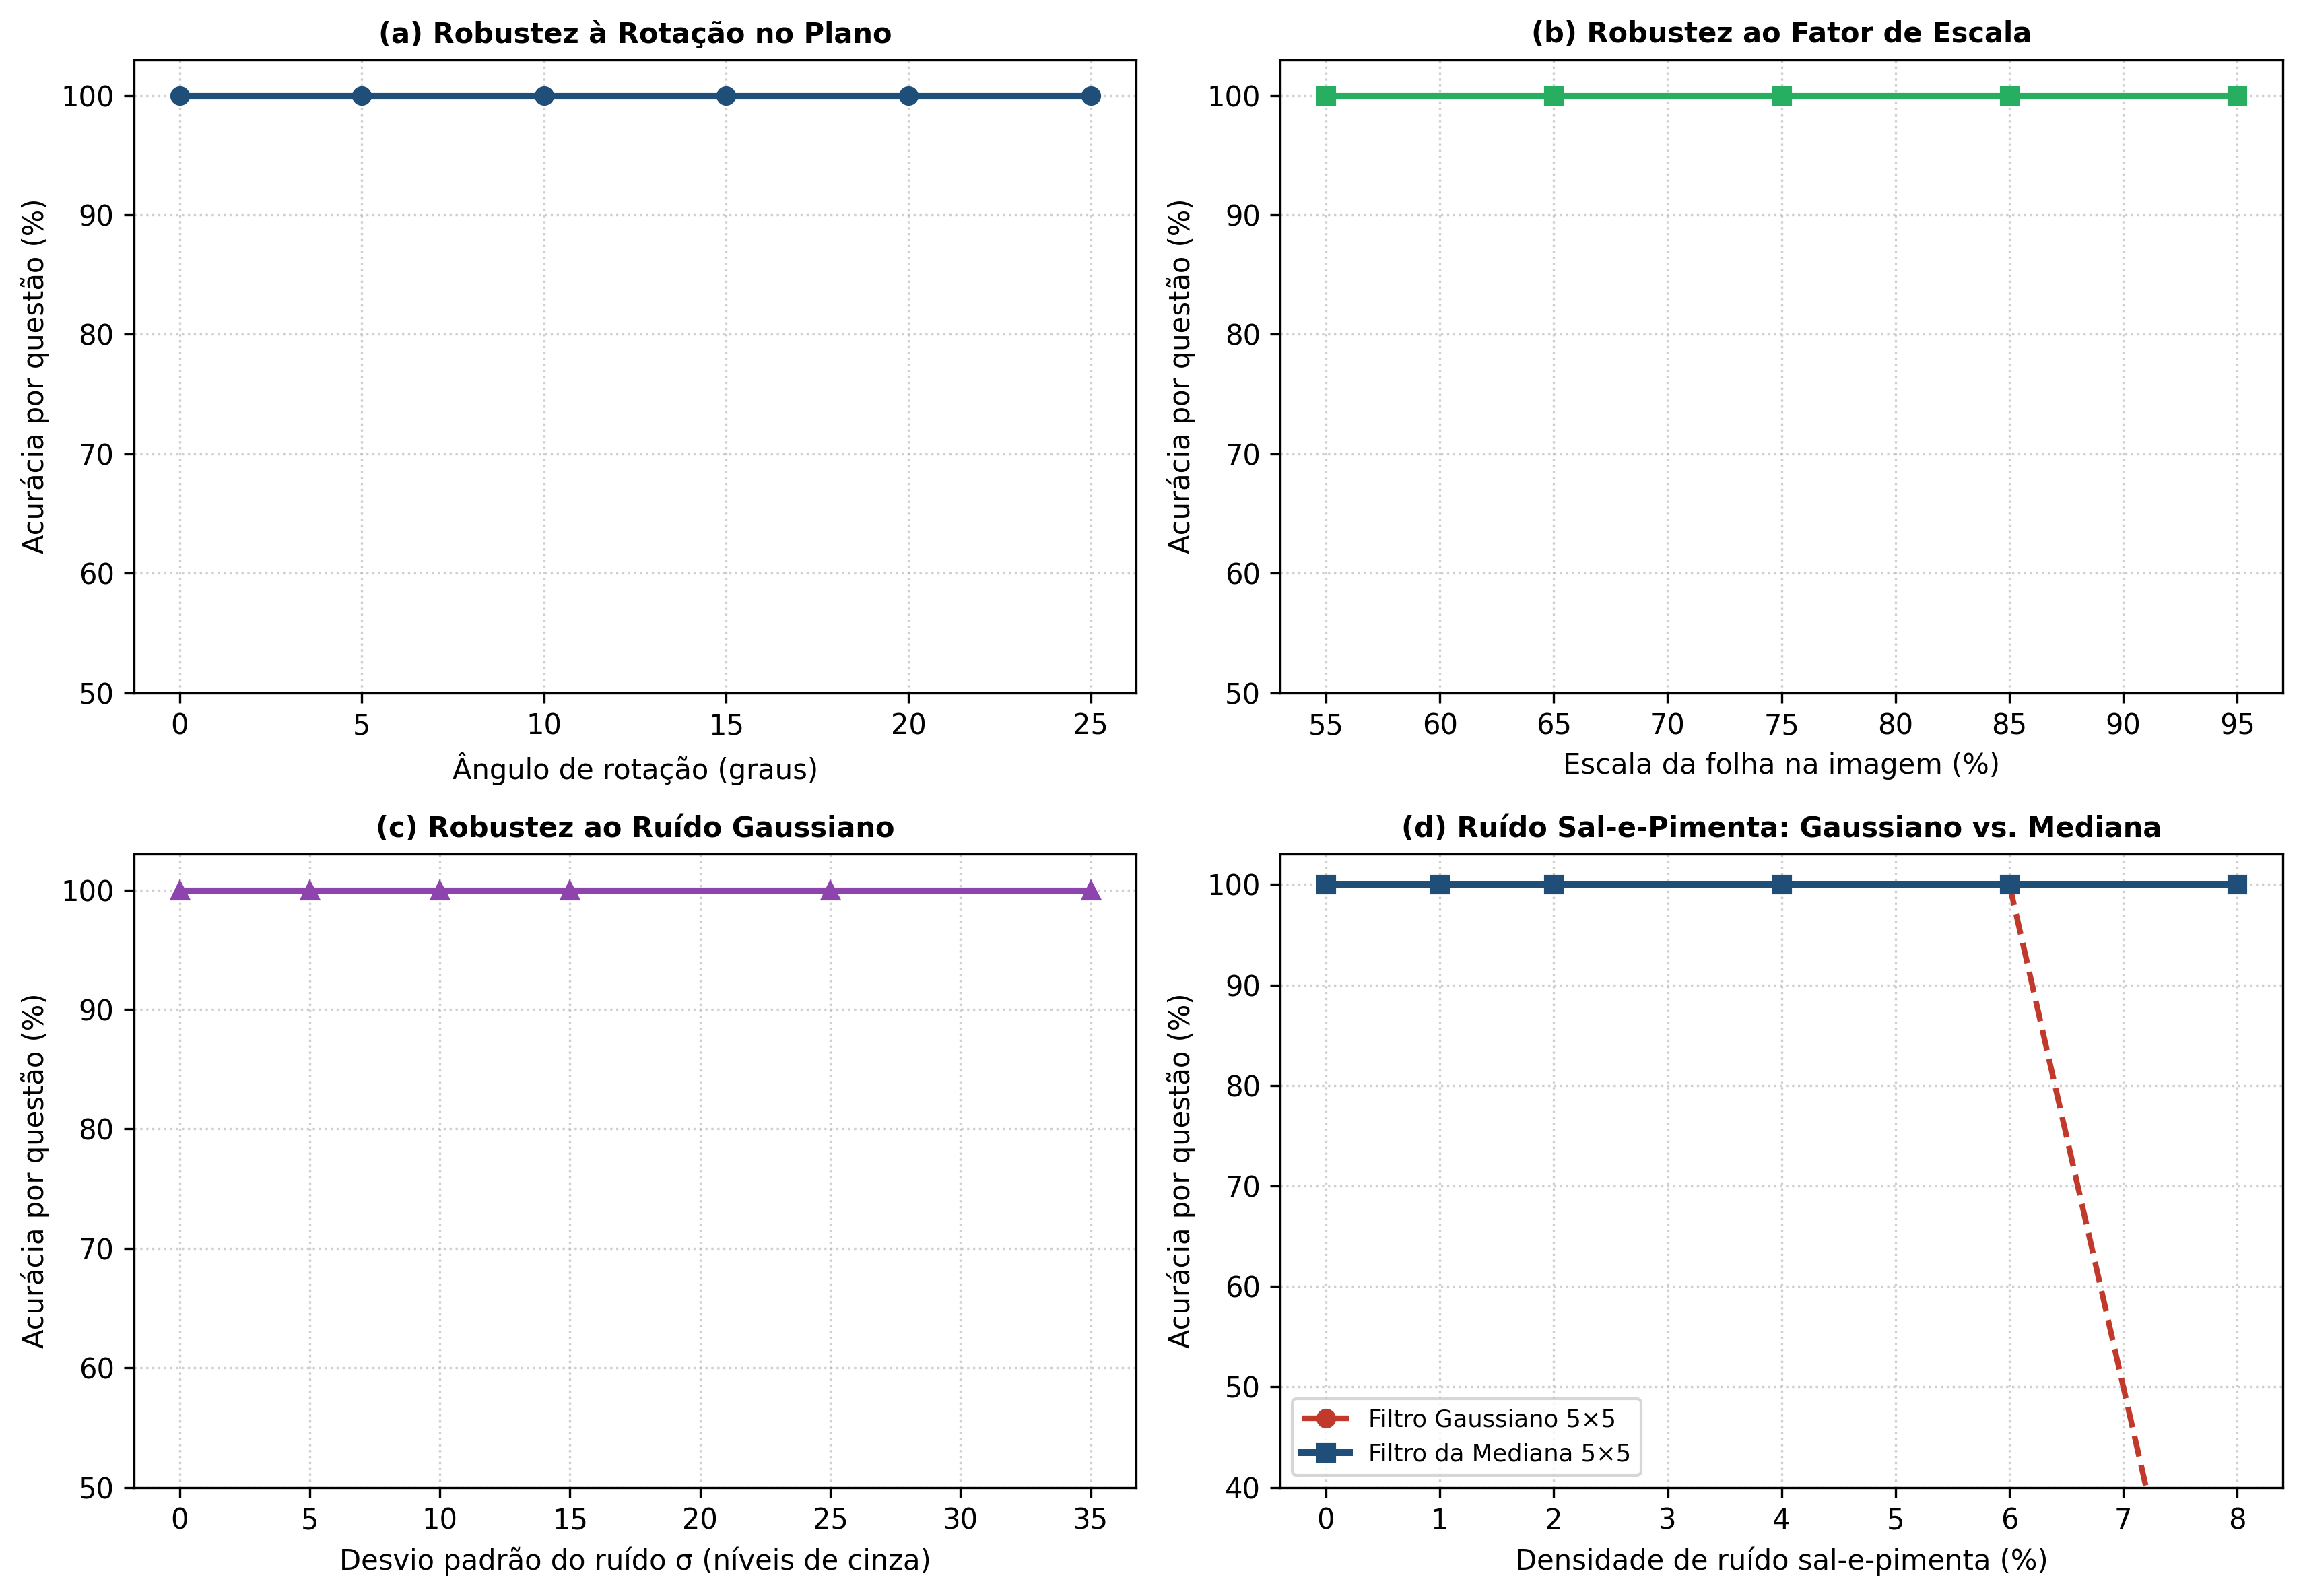
\includegraphics[width=0.92\textwidth]{figuras/fig_curvas_robustez.png}
	\caption{Curvas de robustez paramétrica: (a) ângulo de rotação; (b) fator de escala; (c) ruído Gaussiano ($\sigma$); (d) ruído sal-e-pimenta comparando pré-filtragem Gaussiana vs.\ Mediana.}
	\label{fig:robustez}
\end{figure}

Como limitações críticas e sugestões para continuidade do trabalho, destacam-se: (i) a homografia plana assume que a folha está apoiada sobre uma superfície aproximadamente plana; curvaturas cilíndricas acentuadas (folha segurada na mão no ar) podem deslocar as bolhas centrais em relação à grade projetiva, o que poderia ser mitigado adicionando marcadores fiduciais intermediários ao longo das margens laterais; e (ii) a inclusão de leitura óptica do RA do aluno via grade de dígitos OMR ou QR Code no cabeçalho permitiria associar automaticamente cada nota à pauta da turma.

\bibliography{bibliografia}
\bibliographystyle{plain}

\end{document}
